
%% bare_conf_compsoc.tex
%% V1.4b
%% 2015/08/26
%% by Michael Shell
%% See:
%% http://www.michaelshell.org/
%% for current contact information.
%%
%% This is a skeleton file demonstrating the use of IEEEtran.cls
%% (requires IEEEtran.cls version 1.8b or later) with an IEEE Computer
%% Society conference paper.
%%
%% Support sites:
%% http://www.michaelshell.org/tex/ieeetran/
%% http://www.ctan.org/pkg/ieeetran
%% and
%% http://www.ieee.org/

%%*************************************************************************
%% Legal Notice:
%% This code is offered as-is without any warranty either expressed or
%% implied; without even the implied warranty of MERCHANTABILITY or
%% FITNESS FOR A PARTICULAR PURPOSE! 
%% User assumes all risk.
%% In no event shall the IEEE or any contributor to this code be liable for
%% any damages or losses, including, but not limited to, incidental,
%% consequential, or any other damages, resulting from the use or misuse
%% of any information contained here.
%%
%% All comments are the opinions of their respective authors and are not
%% necessarily endorsed by the IEEE.
%%
%% This work is distributed under the LaTeX Project Public License (LPPL)
%% ( http://www.latex-project.org/ ) version 1.3, and may be freely used,
%% distributed and modified. A copy of the LPPL, version 1.3, is included
%% in the base LaTeX documentation of all distributions of LaTeX released
%% 2003/12/01 or later.
%% Retain all contribution notices and credits.
%% ** Modified files should be clearly indicated as such, including  **
%% ** renaming them and changing author support contact information. **
%%*************************************************************************


% *** Authors should verify (and, if needed, correct) their LaTeX system  ***
% *** with the testflow diagnostic prior to trusting their LaTeX platform ***
% *** with production work. The IEEE's font choices and paper sizes can   ***
% *** trigger bugs that do not appear when using other class files.       ***                          ***
% The testflow support page is at:
% http://www.michaelshell.org/tex/testflow/



\documentclass[conference,compsoc,a4paper]{IEEEtran}
% Some/most Computer Society conferences require the compsoc mode option,
% but others may want the standard conference format.
%
% If IEEEtran.cls has not been installed into the LaTeX system files,
% manually specify the path to it like:
% \documentclass[conference,compsoc]{../sty/IEEEtran}





% Some very useful LaTeX packages include:
% (uncomment the ones you want to load)


% *** MISC UTILITY PACKAGES ***
%
%\usepackage{ifpdf}
% Heiko Oberdiek's ifpdf.sty is very useful if you need conditional
% compilation based on whether the output is pdf or dvi.
% usage:
% \ifpdf
%   % pdf code
% \else
%   % dvi code
% \fi
% The latest version of ifpdf.sty can be obtained from:
% http://www.ctan.org/pkg/ifpdf
% Also, note that IEEEtran.cls V1.7 and later provides a builtin
% \ifCLASSINFOpdf conditional that works the same way.
% When switching from latex to pdflatex and vice-versa, the compiler may
% have to be run twice to clear warning/error messages.

\usepackage[utf8]{inputenc}
\usepackage{bm}
\usepackage{algorithm}
\usepackage[noend]{algpseudocode}
\usepackage{booktabs}
\usepackage{graphicx} 

\usepackage[spanish]{babel}


% *** CITATION PACKAGES ***
%
\ifCLASSOPTIONcompsoc
  % IEEE Computer Society needs nocompress option
  % requires cite.sty v4.0 or later (November 2003)
  \usepackage[nocompress]{cite}
\else
  % normal IEEE
  \usepackage{cite}
\fi
% cite.sty was written by Donald Arseneau
% V1.6 and later of IEEEtran pre-defines the format of the cite.sty package
% \cite{} output to follow that of the IEEE. Loading the cite package will
% result in citation numbers being automatically sorted and properly
% "compressed/ranged". e.g., [1], [9], [2], [7], [5], [6] without using
% cite.sty will become [1], [2], [5]--[7], [9] using cite.sty. cite.sty's
% \cite will automatically add leading space, if needed. Use cite.sty's
% noadjust option (cite.sty V3.8 and later) if you want to turn this off
% such as if a citation ever needs to be enclosed in parenthesis.
% cite.sty is already installed on most LaTeX systems. Be sure and use
% version 5.0 (2009-03-20) and later if using hyperref.sty.
% The latest version can be obtained at:
% http://www.ctan.org/pkg/cite
% The documentation is contained in the cite.sty file itself.
%
% Note that some packages require special options to format as the Computer
% Society requires. In particular, Computer Society  papers do not use
% compressed citation ranges as is done in typical IEEE papers
% (e.g., [1]-[4]). Instead, they list every citation separately in order
% (e.g., [1], [2], [3], [4]). To get the latter we need to load the cite
% package with the nocompress option which is supported by cite.sty v4.0
% and later.





% *** GRAPHICS RELATED PACKAGES ***
%
\ifCLASSINFOpdf
  % \usepackage[pdftex]{graphicx}
  % declare the path(s) where your graphic files are
  % \graphicspath{{../pdf/}{../jpeg/}}
  % and their extensions so you won't have to specify these with
  % every instance of \includegraphics
  % \DeclareGraphicsExtensions{.pdf,.jpeg,.png}
\else
  % or other class option (dvipsone, dvipdf, if not using dvips). graphicx
  % will default to the driver specified in the system graphics.cfg if no
  % driver is specified.
  % \usepackage[dvips]{graphicx}
  % declare the path(s) where your graphic files are
  % \graphicspath{{../eps/}}
  % and their extensions so you won't have to specify these with
  % every instance of \includegraphics
  % \DeclareGraphicsExtensions{.eps}
\fi
% graphicx was written by David Carlisle and Sebastian Rahtz. It is
% required if you want graphics, photos, etc. graphicx.sty is already
% installed on most LaTeX systems. The latest version and documentation
% can be obtained at: 
% http://www.ctan.org/pkg/graphicx
% Another good source of documentation is "Using Imported Graphics in
% LaTeX2e" by Keith Reckdahl which can be found at:
% http://www.ctan.org/pkg/epslatex
%
% latex, and pdflatex in dvi mode, support graphics in encapsulated
% postscript (.eps) format. pdflatex in pdf mode supports graphics
% in .pdf, .jpeg, .png and .mps (metapost) formats. Users should ensure
% that all non-photo figures use a vector format (.eps, .pdf, .mps) and
% not a bitmapped formats (.jpeg, .png). The IEEE frowns on bitmapped formats
% which can result in "jaggedy"/blurry rendering of lines and letters as
% well as large increases in file sizes.
%
% You can find documentation about the pdfTeX application at:
% http://www.tug.org/applications/pdftex





% *** MATH PACKAGES ***
%
\usepackage{amssymb,amsmath} % Math packages for equations
% A popular package from the American Mathematical Society that provides
% many useful and powerful commands for dealing with mathematics.
%
% Note that the amsmath package sets \interdisplaylinepenalty to 10000
% thus preventing page breaks from occurring within multiline equations. Use:
%\interdisplaylinepenalty=2500
% after loading amsmath to restore such page breaks as IEEEtran.cls normally
% does. amsmath.sty is already installed on most LaTeX systems. The latest
% version and documentation can be obtained at:
% http://www.ctan.org/pkg/amsmath





% *** SPECIALIZED LIST PACKAGES ***
%
%\usepackage{algorithmic}
% algorithmic.sty was written by Peter Williams and Rogerio Brito.
% This package provides an algorithmic environment fo describing algorithms.
% You can use the algorithmic environment in-text or within a figure
% environment to provide for a floating algorithm. Do NOT use the algorithm
% floating environment provided by algorithm.sty (by the same authors) or
% algorithm2e.sty (by Christophe Fiorio) as the IEEE does not use dedicated
% algorithm float types and packages that provide these will not provide
% correct IEEE style captions. The latest version and documentation of
% algorithmic.sty can be obtained at:
% http://www.ctan.org/pkg/algorithms
% Also of interest may be the (relatively newer and more customizable)
% algorithmicx.sty package by Szasz Janos:
% http://www.ctan.org/pkg/algorithmicx




% *** ALIGNMENT PACKAGES ***
%
%\usepackage{array}
% Frank Mittelbach's and David Carlisle's array.sty patches and improves
% the standard LaTeX2e array and tabular environments to provide better
% appearance and additional user controls. As the default LaTeX2e table
% generation code is lacking to the point of almost being broken with
% respect to the quality of the end results, all users are strongly
% advised to use an enhanced (at the very least that provided by array.sty)
% set of table tools. array.sty is already installed on most systems. The
% latest version and documentation can be obtained at:
% http://www.ctan.org/pkg/array


% IEEEtran contains the IEEEeqnarray family of commands that can be used to
% generate multiline equations as well as matrices, tables, etc., of high
% quality.




% *** SUBFIGURE PACKAGES ***
%\ifCLASSOPTIONcompsoc
%  \usepackage[caption=false,font=footnotesize,labelfont=sf,textfont=sf]{subfig}
%\else
%  \usepackage[caption=false,font=footnotesize]{subfig}
%\fi
% subfig.sty, written by Steven Douglas Cochran, is the modern replacement
% for subfigure.sty, the latter of which is no longer maintained and is
% incompatible with some LaTeX packages including fixltx2e. However,
% subfig.sty requires and automatically loads Axel Sommerfeldt's caption.sty
% which will override IEEEtran.cls' handling of captions and this will result
% in non-IEEE style figure/table captions. To prevent this problem, be sure
% and invoke subfig.sty's "caption=false" package option (available since
% subfig.sty version 1.3, 2005/06/28) as this is will preserve IEEEtran.cls
% handling of captions.
% Note that the Computer Society format requires a sans serif font rather
% than the serif font used in traditional IEEE formatting and thus the need
% to invoke different subfig.sty package options depending on whether
% compsoc mode has been enabled.
%
% The latest version and documentation of subfig.sty can be obtained at:
% http://www.ctan.org/pkg/subfig




% *** FLOAT PACKAGES ***
%
%\usepackage{fixltx2e}
% fixltx2e, the successor to the earlier fix2col.sty, was written by
% Frank Mittelbach and David Carlisle. This package corrects a few problems
% in the LaTeX2e kernel, the most notable of which is that in current
% LaTeX2e releases, the ordering of single and double column floats is not
% guaranteed to be preserved. Thus, an unpatched LaTeX2e can allow a
% single column figure to be placed prior to an earlier double column
% figure.
% Be aware that LaTeX2e kernels dated 2015 and later have fixltx2e.sty's
% corrections already built into the system in which case a warning will
% be issued if an attempt is made to load fixltx2e.sty as it is no longer
% needed.
% The latest version and documentation can be found at:
% http://www.ctan.org/pkg/fixltx2e


%\usepackage{stfloats}
% stfloats.sty was written by Sigitas Tolusis. This package gives LaTeX2e
% the ability to do double column floats at the bottom of the page as well
% as the top. (e.g., "\begin{figure*}[!b]" is not normally possible in
% LaTeX2e). It also provides a command:
%\fnbelowfloat
% to enable the placement of footnotes below bottom floats (the standard
% LaTeX2e kernel puts them above bottom floats). This is an invasive package
% which rewrites many portions of the LaTeX2e float routines. It may not work
% with other packages that modify the LaTeX2e float routines. The latest
% version and documentation can be obtained at:
% http://www.ctan.org/pkg/stfloats
% Do not use the stfloats baselinefloat ability as the IEEE does not allow
% \baselineskip to stretch. Authors submitting work to the IEEE should note
% that the IEEE rarely uses double column equations and that authors should try
% to avoid such use. Do not be tempted to use the cuted.sty or midfloat.sty
% packages (also by Sigitas Tolusis) as the IEEE does not format its papers in
% such ways.
% Do not attempt to use stfloats with fixltx2e as they are incompatible.
% Instead, use Morten Hogholm'a dblfloatfix which combines the features
% of both fixltx2e and stfloats:
%
% \usepackage{dblfloatfix}
% The latest version can be found at:
% http://www.ctan.org/pkg/dblfloatfix




% *** PDF, URL AND HYPERLINK PACKAGES ***
%
%\usepackage{url}
% url.sty was written by Donald Arseneau. It provides better support for
% handling and breaking URLs. url.sty is already installed on most LaTeX
% systems. The latest version and documentation can be obtained at:
% http://www.ctan.org/pkg/url
% Basically, \url{my_url_here}.




% *** Do not adjust lengths that control margins, column widths, etc. ***
% *** Do not use packages that alter fonts (such as pslatex).         ***
% There should be no need to do such things with IEEEtran.cls V1.6 and later.
% (Unless specifically asked to do so by the journal or conference you plan
% to submit to, of course. )


% correct bad hyphenation here
\hyphenation{op-tical net-works semi-conduc-tor}


\begin{document}
%
% paper title
% Titles are generally capitalized except for words such as a, an, and, as,
% at, but, by, for, in, nor, of, on, or, the, to and up, which are usually
% not capitalized unless they are the first or last word of the title.
% Linebreaks \\ can be used within to get better formatting as desired.
% Do not put math or special symbols in the title.
\title{Una Metaheurística GRASP para Integración en Grafos}


% author names and affiliations
% use a multiple column layout for up to three different
% affiliations
\author{
\IEEEauthorblockN{Manuel Dubinsky}
\IEEEauthorblockA{Ingeniería Informática\\
Dpto. Tecnología y Administración\\
Universidad Nacional de Avellaneda\\
Argentina}
\and
\IEEEauthorblockN{César Massri}
\IEEEauthorblockA{Dpto. de Matemática\\
Universidad de CAECE,\\
IMAS, CONICET\\
Argentina}
\and
\IEEEauthorblockN{Fernando Asteasuain}
\IEEEauthorblockA{Ingeniería Informática\\
Dpto. Tecnología y Administración\\
Universidad Nacional de Avellaneda\\
Argentina}
}

% conference papers do not typically use \thanks and this command
% is locked out in conference mode. If really needed, such as for
% the acknowledgment of grants, issue a \IEEEoverridecommandlockouts
% after \documentclass

% for over three affiliations, or if they all won't fit within the width
% of the page (and note that there is less available width in this regard for
% compsoc conferences compared to traditional conferences), use this
% alternative format:
% 
%\author{\IEEEauthorblockN{Michael Shell\IEEEauthorrefmark{1},
%Homer Simpson\IEEEauthorrefmark{2},
%James Kirk\IEEEauthorrefmark{3}, 
%Montgomery Scott\IEEEauthorrefmark{3} and
%Eldon Tyrell\IEEEauthorrefmark{4}}
%\IEEEauthorblockA{\IEEEauthorrefmark{1}School of Electrical and Computer Engineering\\
%Georgia Institute of Technology,
%Atlanta, Georgia 30332--0250\\ Email: see http://www.michaelshell.org/contact.html}
%\IEEEauthorblockA{\IEEEauthorrefmark{2}Twentieth Century Fox, Springfield, USA\\
%Email: homer@thesimpsons.com}
%\IEEEauthorblockA{\IEEEauthorrefmark{3}Starfleet Academy, San Francisco, California 96678-2391\\
%Telephone: (800) 555--1212, Fax: (888) 555--1212}
%\IEEEauthorblockA{\IEEEauthorrefmark{4}Tyrell Inc., 123 Replicant Street, Los Angeles, California 90210--4321}}




% use for special paper notices
%\IEEEspecialpapernotice{(Invited Paper)}



% make the title area
\maketitle

% As a general rule, do not put math, special symbols or citations
% in the abstract

\renewcommand\abstractname{Abstract}

\begin{abstract}

Given an edge-weighted graph, we analyze the problem of finding an 
orientation of its edges and a function on its nodes, such that 
for each oriented edge the consistent subtraction of the function on 
its incident vertices (ie.: head - tail), is the best approximation in 
a least square sense to the original edge-weighted function. We 
present a simple GRASP algorithm to find a ``good" \ solution that is 
suitable for distributed execution.

\end{abstract}

% no keywords




% For peer review papers, you can put extra information on the cover
% page as needed:
% \ifCLASSOPTIONpeerreview
% \begin{center} \bfseries EDICS Category: 3-BBND \end{center}
% \fi
%
% For peerreview papers, this IEEEtran command inserts a page break and
% creates the second title. It will be ignored for other modes.
\IEEEpeerreviewmaketitle



\section{Introducción}
\subsection{Descripción del problema}

Dado un grafo conexo $G=(V,E)$ \cite{Harari:1969} y una función 
de pesos en los ejes $f: E \rightarrow \mathbb{R}$, queremos hallar 
una orientación de los ejes de $G$ y una función de pesos en los 
nodos $x: V \rightarrow \mathbb{R}$ de modo 
de minimizar el error:

$$E(x) := \sum_{e \in E} (dx(e) - f(e))^2$$

\noindent donde $dx: E \rightarrow \mathbb{R}$ es el \textit{diferencial} de $x$ 
(asociado a la orientación de los ejes) y se define en cada eje 
$e=v\to w$ como $dx(e) = x(w) - x(v)$.

\smallskip

Concretamente, si consideramos la correspondencia entre orientaciones 
de $G$ y \textit{matrices de incidencia dirigida}, se trata de 
encontrar: por un lado la ``mejor'' \textit{matriz de incidencia 
dirigida} $D$, y por el otro la mejor función de pesos en los ejes 
$x: V \rightarrow \mathbb{R}$ de modo de minimizar la expresión:

$$E(x) = \|D\bm{x}-\bm{f}\|^2$$

\noindent donde:

$$
\bm{x} = 
\begin{bmatrix}
	x(v_1)\\
	\dots \\
	x(v_n)
\end{bmatrix}, 
\bm{f} = 
\begin{bmatrix}
	f(e_1)\\
	\dots \\
	f(e_m)
\end{bmatrix}
$$

El algoritmo que proponemos explora el espacio de todas las 
orientaciones posibles del grafo original.

\subsection{Contexto del problema y trabajos relacionados}
El problema surgió a partir de la definición de \textit{1-forma 
diferencial} en el contexto de \textit{mallas poligonales}. 

\bigskip

Las formas diferenciales \cite{S:1965,T:2008} conceptualizan la noción 
de objeto integrable. Son objetos de estudio en geometría diferencial. 
Intuitivamente se puede pensar en una 
\textit{1-forma diferencial} como una cantidad que mide 
una distancia infinitesimal y que puede ser integrada a lo largo de una 
curva. Análogamente una \textit{2-forma diferencial} es una cantidad 
que mide una superficie infinitesimal y que puede ser integrada a lo 
largo de una superficie. Y en general, una \textit{k-forma diferencial} 
está asociada a una variedad diferencial $k$-dimensional y puede ser 
integrada en dimensión $k$. Esta noción permite unificar varios 
teoremas clásicos como el \textit{teorema de Green} y el \textit{teorema 
de Stokes}. Además de la naturaleza geométrica de este punto de vista, 
las formas diferenciales tienen una rica estructura algebraica que 
permite entre otras cosas trasladar propiedades invariantes entre dos 
variedades mediante mapas diferenciales. El precursor de la 
teoría fue el matemático francés \textit{Elie Cartan} a fines del siglo 
XIX.

\bigskip

Por otro lado, las \textit{mallas poligonales} 
\cite{BKPAL:2010} permiten representar superficies inmersas en el 
espacio tridimensional. Están compuestas por aproximaciones lineales 
poligonales de pequeñas vecindades de la superficie denominadas caras. 
Y tienen asociado un grafo cuyos nodos y ejes definen los vértices y 
lados de las caras. Son objetos de estudio fundamentales en el área de 
\textit{procesamiento digital de geometría}. Esta área ha crecido de 
manera sostenida en los últimos veinte años debido a la capacidad de 
obtener modelos geométricos de objetos reales mediante técnicas como: 
tomografía computarizada, resonancia magnética, escaneo mediante láser y 
ultrasonido, y microscopía. Numerosas disciplinas como la medicina, la 
ingeniería, la astrofísica, la exploración geográfica, la arquitectura 
y el urbanismo, como así también las industrias cinematográfica, de 
videojuegos, y de fabricación de manufacturas se nutren continuamente 
de modelos tridimensionales. El área de \textit{procesamiento digital 
de geometría} es la encargada de proveer herramientas y aplicaciones 
para producir dichos modelos. Las aplicaciones son muy variadas, 
algunos ejemplos son: escaneo 3D 
\cite{LRAT:2008}, navegación de vehículos autónomos \cite{CMT:2008}, 
reconocimiento de patrones \cite{TC:1992}, 
reconocimiento de trayectorias \cite{ZT:2009}, construcción de modelos 
tridimensionales de sitios arqueológicos \cite{REVEAL}, de esculturas 
y objetos antiguos \cite{BMMRT:2002}, cinematografía 3D 
\cite{RT:2007}, etc.

\bigskip

La teoría de formas diferenciales tiene su contraparte discreta en el 
marco de las mallas poligonales. Esto se debe a que una malla poligonal 
puede ser entendida como una descomposición simplicial 
\cite{Hatcher:2004} de la superficie que está modelando. Y una forma 
diferencial puede interpretarse como un complejo de co-cadena sobre 
dicha descomposición. En el trabajo \cite{DKT:2006}, los autores 
muestran cómo integrar formas diferenciales mediante una técnica de 
interpolación. En ese contexto los $1$-símplices de la descomposición, 
o dicho de otro modo: los ejes del grafo asociado a la malla, ya están 
dotados de una orientación. Y están sujetos a la equivalencia 
${v_0v_1} = -{v_1v_0}$, es decir que si se considera la orientación 
contraria de un eje, su término asociado en el complejo de co-cadena 
cambia de signo (esto es compatible con el primer teorema fundamental 
del cálculo). 

\bigskip

El problema que consideramos en este trabajo es una variante en la 
cual los ejes del grafo subyacente no están dotados de una orientación. 
El problema de optimización consiste justamente en encontrar una 
orientación que ajuste del mejor modo posible los valores de los 
vértices de acuerdo a una función de pesos en los ejes del grafo.


\subsection{Aplicaciones}

Las aplicaciones son aquellas en las cuales necesitamos construir una 
función de los nodos que respete ciertas restricciones diferenciales.

Por ejemplo, supongamos que los nodos representan regiones geográficas 
y queremos construir un mapa topográfico basado en ciertas relaciones 
diferenciales de altura entre algunas regiones.

Otro ejemplo es el de ordenar cronológicamente ciertos eventos 
en base a algunas relaciones diferenciales entre ellos.

\section{Preliminares}

\subsection{Álgebra lineal}

\textbf{La \textit{matriz de incidencia dirigida}}

\smallskip

La \textit{matriz de incidencia dirigida} ($D$) de un grafo dirigido 
$\vec G = (\vec V, \vec E)$ es una matriz de $m \times n$ (donde $|\vec
 E| = m$ y $|\vec V| = n$) tal que para cada eje orientado 
$e_k=v_i \rightarrow v_j$: $D_{ki} = -1$, $D_{kj} = 1$ y vale $0$ en 
las demás entradas de la fila $k$.

\smallskip

En otros términos, una matriz de incidencia dirigida representa una 
 orientación de los ejes de un grafo no dirigido $G$. Y el 
espacio de matrices de incidencia dirigida asociado a $G$ 
equivale al espacio de todas las orientaciones posibles de $G$.

\bigskip

\noindent{\textbf{La \textit{matriz laplaciana}}}

La \textit{matriz laplaciana} ($L$) de un grafo $G$ es una matriz de 
$n \times n$ definida del siguiente modo:

$$
	L_{ij} =
	\begin{cases}
	deg(v_i) & \text{si $i = j$} \\
	-1 & \text{si existe el eje $(v_i,v_j)$} \\
	0 & \text{en otro caso} 
	\end{cases}
$$

El rango de $L$ es $n-c$ donde $c$ es la cantidad de componentes 
conexas. En particular si $G$ es conexo, el rango de $L$ es $n-1$

\bigskip

\noindent{\textbf{Relación entre las matrices $L$ y $D$}}

Es fácil verificar que las matrices $L$ y $D$ se relacionan de acuerdo
a la expresión:

$$L = D^t D$$

Es importante notar que $L$ es independiente de cualquier orientación 
que se le asocie al grafo. Y que el rango de $D$ es el mismo que el de 
$L$. Como en nuestro caso $G$ es conexo el rango de $D$ es $n-1$.

\bigskip

\noindent{\textbf{Sistema lineal inducido por $D$}}

Recordemos que el problema que queremos resolver es encontrar la matriz 
de incidencia dirigida $D$, es decir la ``mejor'' 
orientación de los ejes 
del grafo $G$, de modo de minimizar la expresión:

$$E(x) = \|D\bm{x}-\bm{f}\|^2$$

Para eso será preciso explorar el espacio de matrices de 
incidencia dirigida asociado a $G$. Una vez que conseguimos una 
matriz candidata, el problema de minimización es equivalente a encontrar
dónde se anula el gradiente de $E(x)$:
 
$$\nabla E = \left[\frac{\partial E}{\partial x_1}, \dots, \frac{\partial 
E}{\partial x_n}\right] = D^tDx-D^tf=0$$

\noindent Que a su vez es equivalente a resolver el sistema lineal:

$$D^tDx = Lx = D^tf$$

Mediante métodos iterativos es posible converger al punto más cercano 
al vector $D^tf$ contenido en el subespacio generado por $L$ (la 
proyección ortogonal de $D^tf$). Específicamente en este trabajo 
emplearemos el método de \textit{Gradiente Conjugado} \cite{Saad:2007} 
para resolver el sistema lineal.

\smallskip

Es importante mencionar que en el último 
tiempo ha habido grandes avances en la creación de nuevos métodos 
iterativos para resolver esta clase particular de sistemas lineales 
(aquellos que involucran una matriz laplaciana) denominados 
\textit{sistemas laplacianos} (\cite{KMP:2010,Spielman:2010,ST:2004,
Teng:2010}).

\bigskip

\noindent{\textbf{Norma de la proyección ortogonal}}

Para elaborar el criterio que nos permita comparar dos matrices de 
incidencia dirigida y decidir cuál es mejor en el contexto del problema 
que queremos resolver, vamos a referirnos a nociones básicas de 
proyección ortogonal de un vector sobre un subespacio de un espacio 
vectorial, \cite{WK:2009}.

\smallskip

Sean $v,w \in \mathbb{R}^n$, notamos $p_v(w)$ a la proyección de $w$ 
sobre $v$. Mediante relaciones trigonométricas básicas podemos 
calcular $\|p_v(w)\|$ (la norma de $p_v(w)$):

$$\frac{|v w|}{\|w\|} = \frac{|cos(\alpha)| \ \|v\| \ \|w\|}{\|w\|} = 
|cos(\alpha)| \ \|v\| = \|p_v(w)\|$$

De modo más general, notamos $p_S(w)$ a la proyección ortogonal de $w$
sobre un subespacio $S \subset \mathbb{R}^n$ generado por una base 
ortogonal $S = \langle s_1, \dots, s_k\rangle $. La norma de $p_S(w)$ puede calcularse
de modo análogo:

$$
\|p_S(w)\| = \|\begin{bmatrix}
	\|p_{s_1}(w)\| \\
	\dots \\
	\|p_{s_k}(w)\|
\end{bmatrix}\|
$$

\smallskip

Para dar una intuición geométrica del hecho precedente, supongamos (sin 
pérdida de generalidad) que $S = \langle e_1, \dots, e_k\rangle $ está dada por los 
primeros $k$ vectores canónicos y $w = (w_1, \dots, w_n)$. 
Claramente la proyección ortogonal de $w$ sobre $S$ es 
$(w_1, \dots, w_k)$ (las primeras $k$ componentes de $w$). Entonces 
verifiquemos la expresión anterior:

$$
\|\begin{bmatrix}
	\|p_{s_1}(w)\| \\	
	\dots \\
	\|p_{s_k}(w)\|
\end{bmatrix}\| = 
\|\begin{bmatrix}
	|cos(\alpha_1)| \ \|w\| \\
	\dots \\
	|cos(\alpha_k)| \ \|w\|
\end{bmatrix}\| = 
\|\begin{bmatrix}
	w_1 \\
	\dots \\
	w_k
\end{bmatrix}\|
$$

\smallskip

Informalmente, el caso general se puede reducir a este caso simple 
mediante una matriz rotación, que preserva las normas.

\subsection{Metaheurísticas}

En el contexto del tratamiento de problemas de complejidad $NP$, el 
enfoque metaheurístico (\cite{GP:2010,Talbi:2009}) procura encontrar buenas soluciones (no 
necesariamente las mejores) en tiempo polinomial. Algunas 
metaheurísticas son:

\begin{itemize}
	\item Simulated-annealing
	\item Tabu-search
	\item GRASP
	\item Algoritmos genéticos
	\item Colonia de hormigas
\end{itemize}

Encontrar la metaheurística más adecuada depende del problema que se 
quiera resolver y debe ser contrastada empíricamente con los resultados 
obtenidos por otras metaheurísticas.

\smallskip

Específicamente una metaheurística de tipo \textit{GRASP} combina dos 
aspectos. Por un lado, requiere cierto tipo de búsqueda local, es decir: 
explorar un entorno de la solución de la iteración actual, para lo cual 
es preciso definir una noción de vecindad en el espacio; en nuestro caso 
se tratará de definir una noción de vecindad en el espacio de matrices 
de incidencia dirigida asociado a un grafo. Y por otro lado, GRASP 
requiere cierto grado de azar en la elección del vecino a explorar en 
la siguiente iteración; esto busca impedir que el algoritmo se 
estabilice entorno a un mínimo local (no necesariamente un mínimo 
global). 

\smallskip

En la próxima sección se presentará el algoritmo y se describirán las 
particularidades de la implementación de una metaheurística GRASP en el 
contexto del problema que queremos resolver.

\section{Implementación}

En esta sección describiremos el algoritmo y los detalles de la 
implementación.

\subsection{La ``mejor'' matriz de incidencia dirigida}

El primer paso de la estrategia que vamos a desarrollar es tratar de 
encontrar la ``mejor'' matriz de incidencia dirigida, o dicho en otros 
términos: de orientar los ejes del grafo $G$ del mejor modo posible para 
minimizar el error:

$$E(x) = \|D\bm{x}-\bm{f}\|^2$$
 
Como el espacio de matrices de incidencia dirigida asociado a $G$ es un 
espacio de tamaño exponencial respecto a la cantidad de ejes, dado que 
cada eje puede tener dos orientaciones, nuestra propuesta está centrada 
en construir un algoritmo que devuelva la ``mejor solución posible''.

\bigskip

\noindent{\textbf{Preprocesamiento de las hojas del grafo}}

Inicialmente proponemos un preprocesamiento del grafo con el objetivo de 
simplificarlo. En la formulación del problema de minimización:

$$E(x) = \|D\bm{x}-\bm{f}\|^2 = \sum_{e \in E} (dx(e) - f(e))^2$$

Consideremos una hoja $v$ de $G$ (un nodo de grado 1), a su único 
vecino $w$ y al eje que los liga $e=(v,w)$. Dependiendo de la 
orientación de $e$, surge que $x(v) = x(w) \pm 
f(e)$, es decir que $x(v)$ queda determinado por $x(w)$, $f(e)$ y la 
elección de una orientación de $e$.

\smallskip

Por lo tanto, es posible reducir el grafo original $G$, eliminando 
recursivamente sus  hojas de modo de obtener un grafo más simple (un 
grafo con menos ejes y nodos):

\begin{verbatim}
         while (G has leaves) {
             G = stripLeaves(G);
         }
\end{verbatim}

Un corolario es que si $G$ es un árbol, entonces $x: V 
\rightarrow \mathbb{R}$ queda determinada por alguna orientación de 
los ejes y por $x(v)$ para un nodo $v$.

\smallskip

De ahora en adelante consideraremos que el grado de los nodos de $G$ es 
al menos 2.
 
\bigskip

\noindent{\textbf{Una base semi-ortogonal}}

Un hecho simple que se deriva de la expresión que vincula a las matrices 
$L$ y $D$:

$$L = D^t D$$

\noindent es que el producto interno de dos columnas distintas de una matriz de 
incidencia dirigida vale $-1$ o $0$ dependiendo de si existe un eje 
entre los nodos asociados a dichas columnas o no. Notar el hecho 
evidente de que si el producto es $0$, las columnas son
 ortogonales.

\smallskip

Ahora notemos lo siguiente: si G es conexo, el ángulo entre dos 
columnas $d_i$ y $d_j$ de $D$ está contenido en el rango 
$[\frac{\pi}{2},\frac{2\pi}{3}]$. Para ver esto, supongamos que existe 
un eje entre los nodos $v_i$ y $v_j$ asociados a dichas columnas. 
El ángulo puede medirse de este modo:

$$cos(\alpha) \ \|d_i\| \ \|d_j\|= d_i  d_j \implies cos(\alpha) = 
\frac{d_i d_j}{\|d_i\| \ \|d_j\|}$$

El módulo de esta fracción se maximiza cuando las normas de las 
columnas son más pequeñas o de modo equivalente: cuando los grados de 
los nodos correspondientes se minimizan. Respecto a esta última 
observación, cabe aclarar que la norma de cada columna de $D$ es igual 
al grado del nodo asociado a esa columna, esto se deduce de la diagonal 
de $L = D^t D$. Recordemos que el grado de cada nodo de  $G$, luego de 
preprocesar las hojas, es al menos 2. Entonces resulta que:

$$-\frac{1}{2}\le cos \ \alpha = \frac{d_i d_j}{\|d_i\| \ \|d_j\|} \le 0,\quad \forall i\neq j.$$

\smallskip

\noindent Implicando que $\frac{\pi}{2}\le\alpha \leq \frac{2\pi}{3}$.

\smallskip

Denotaremos base \textit{semi-ortogonal} a una base (de un 
$\mathbb{R}$-espacio vectorial) tal que el ángulo entre cualquier par de 
generadores está en el rango $[\frac{\pi}{2},\frac{2\pi}{3}]$.

\smallskip

El hecho de que las columnas de una matriz de incidencia dirigida 
definan una base semi-ortogonal va a justificar el criterio que 
emplearemos para compararlas.

\bigskip

\noindent{\textbf{La \textit{$\alpha$-norma}. Un criterio para comparar 
matrices de incidencia dirigida}}

Una interpretación geométrica del problema de minimización que queremos 
resolver es la siguiente: encontrar la ``mejor'' matriz de incidencia 
dirigida $D$ tal que la distancia de $f$ sobre el subespacio 
generado por las columnas de $D$ sea mínima. En el caso de que 
el vector $f$ esté contenido en el subespacio, entonces el problema 
tiene solución exacta, es decir: el sistema lineal $Dx = f$ tiene 
solución.

\smallskip

Para resolver el problema, necesitamos un criterio para comparar  
matrices de incidencia dirigida asociadas al grafo $G$. Como las 
columnas de una matriz de incidencia dirigida $D$ definen una base 
semi-ortogonal, aproximaremos la norma de la proyección 
ortogonal de $f$ sobre $D$ como si las columnas de $D$ fueran 
ortogonales y denotaremos a esta aproximación \textit{$\alpha$-norma}.
 De este modo, entre dos matrices de incidencia dirigida $D$ y 
 $\bar{D}$ nuestro criterio será optar por aquella con mayor 
 $\alpha$-norma. La justificación de esta decisión se basa en que 
 calcular una base ortonormal del subespacio generado por las columnas 
 de $D$, mediante por ejemplo el método de \emph{Gram-Schmidt} 
 \cite{WK:2009} no es viable en términos de costo computacional.

\smallskip

La $\alpha$-norma se puede calcular en dos pasos. El paso inicial sería 
calcular el producto interno de $f$ con las columnas de $D$:

$$
D^t f = \begin{bmatrix}
	cos(\alpha_1) \ \|d_1\| \ \|f\|\\
	\dots \\
	cos(\alpha_n) \ \|d_n\| \ \|f\|
\end{bmatrix}
$$

\smallskip

Y luego dividir cada componente por la norma correspondiente:

$$
\alpha(D,f) = \| D^t f
\begin{bmatrix}
	\|d_1\|^{-1}\\
	\dots \\
	\|d_n\|^{-1} 
\end{bmatrix} \|= \|\begin{bmatrix}
	cos(\alpha_1) \ \|f\|\\
	\dots \\
	cos(\alpha_n) \ \|f\|
\end{bmatrix}\|
$$

\smallskip

Notemos que para cambiar la dirección de un eje en una matriz de 
incidencia dirigida $D$, hay que cambiarle el signo a la fila correspondiente al 
eje que se quiere modificar. Y de modo más general, si queremos cambiar 
la dirección de varios ejes simultáneamente la nueva matriz $\bar{D}$
se puede calcular del siguiente modo:

$$\bar{D} = \bar{I} D$$

\smallskip

\noindent donde $\bar{I}$ es la matriz diagonal de $m \times m$ que tiene un $-1$ 
en cada fila asociada a cada eje que queremos invertir y $1$ en el resto 
de sus componentes.

\smallskip

Notemos que la norma de las columnas de $D$ y $\bar{D}$ son iguales 
porque sólo difieren en el signo de algunas componentes. Por lo tanto, 
la norma de las columnas de las matrices de incidencia dirigida puede 
calcularse una sola vez. 
%En conclusión, obtenemos la identidad,
%\[
%\alpha(\bar{I}D,f)=\bar{I}\alpha(D,f).
%\]




\bigskip

\subsection{El enfoque metaheurístico}

El problema que queremos resolver se traduce en encontrar una matriz de 
incidencia dirigida $D$ que maximice la $\alpha$-norma de $f$. 
Dado que el tamaño del espacio de matrices de 
incidencia dirigida es $2^m$  (donde $|E|=m$), computar el problema
para grafos de tamaño grande es difícil de resolver. 
Este espacio es 
extremadamente grande incluso para grafos pequeños. Por lo tanto, el 
problema admite un enfoque metaheurístico que nos permita encontrar 
una solución ``buena'' (aunque no necesariamente la mejor).

\smallskip

Como ya mencionamos, las metaheurísticas \textit{GRASP} combinan azar y 
búsqueda local. La búsqueda local se refiere a la exploración de 
una vecindad de un punto del espacio. En nuestro caso el espacio es el 
conjunto de matrices de incidencia dirigida asociado a $G$. Una 
definición obvia de vecindad de una matriz de incidencia dirigida $D$ es 
el conjunto de matrices que difieren en la dirección de un eje, o sea 
aquellas que tienen una fila invertida con respecto a $D$. Cada vez que 
se encuentra un mínimo (o máximo), lo conservamos. La sencillez de 
GRASP y la posibilidad de paralelizarlo de un modo natural, lo 
convierten en una alternativa razonable para nuestro problema.

\subsection{El algoritmo}

La estrategia que presenta nuestro algoritmo es una variante en la que 
invertimos los aspectos de azar y búsqueda local de \textit{GRASP}: 
primero elegimos al azar un conjunto de vecinos y luego definimos como 
nuevo punto a explorar al mejor de ellos (el que tenga mayor 
$\alpha$-norma). 

\smallskip

El algoritmo está controlado por dos parámetros:

\begin{itemize}
	\item La vecindad de un punto está determinada por el parámetro 
	$\phi$, que establece la cantidad de ejes del punto que deben 
	modificarse al azar para construir un vecino.
	\item La cantidad de vecinos del punto que debemos explorar en cada 
	iteración está dada por el parámetro $\psi$
\end{itemize}

A continuación presentamos el pseudocódigo del algoritmo y luego 
comentamos las funciones auxiliares.

\begin{algorithm}
    \caption{Integrate($G,f,\phi,\psi$)}
	\begin{algorithmic}
		\State $currentPoint \gets Initialize(G)$
		\State $bestPoint \gets currentPoint$
		\While{p}
			\State $\Omega \gets Neighbors(currentPoint)$
			\State $bestNeighbor \gets BestNeighbor(\Omega,f)$
			\If{$\alpha(bestNeighbor,f)>\alpha(bestPoint,f)$}
				\State $bestPoint \gets bestNeighbor$
			\EndIf
			\State $currentPoint \gets bestNeighbor$
		\EndWhile
		\State Solve laplacian system $L x = D^t f$ \\
		\Return $x$
	\end{algorithmic}
	\label{alg:alg1}
\end{algorithm}

La función \emph{Initialize(G)} se encarga de construir 
una matriz de incidencia dirigida inicial. Concretamente la orientación 
de los ejes de esa matriz se define desde el nodo con menor 
etiqueta al de mayor a partir de un etiquetado previo de los nodos del 
grafo. 

\smallskip

La función \emph{Neighbors(currentPoint)} devuelve un conjunto de 
vecinos del punto que se está explorando en la iteración. El conjunto 
de vecinos se arma en base a los parámetros $\phi$ y $\psi$. El 
resultado es un conjunto de $\psi$ vecinos cada uno de los cuales 
difiere en la dirección de exactamente $\phi$ ejes (elegidos al azar) 
con respecto $currentPoint$.

\smallskip

La función $BestNeighbor(\Omega,f)$ devuelve el mejor vecino del conjunto 
de entrada. O sea, aquel que tiene mayor $\alpha$-norma. Y por último, 
la función $\alpha(bestNeighbor,f)$ calcula la $\alpha$-norma de la matriz 
de incidencia de entrada.

\smallskip

La condición de corte del $While$ es un predicado ($p$) que permite 
terminar la ejecución por criterios distintos: cantidad de iteraciones, 
tiempo de ejecución transcurrido, margen de error de la mejor solución 
encontrada dentro de un rango de aceptación.

\smallskip

Y por último, el sistema laplaciano ($Lx = D^t f$) se resuelve mediante 
el método de \emph{Gradiente Conjugado}.

\section{Resultados}

En esta sección describimos los resultados obtenidos. Primero 
comentamos el criterio que adoptamos para determinar los valores de los 
parámetros $\phi$ y $\psi$. Y posteriormente nos enfocamos en el 
análisis del algoritmo evaluado sobre tres familias de grafos: 

\begin{itemize}
	\item \emph{Grafos completos}: son aquellos en los que todo par de  
	nodos está ligado por un eje.
	\item \emph{Ciclos simples}: grafo que define un ciclo sin ciclos 
	propios; se puede pensar en un polígono simple como modelo 
	geométrico.
	\item \emph{Mallas poligonales}: son representaciones de superficies 
	inmersas en el espacio tridimensional; tienen más estructura que un 
	grafo porque los nodos tienen asociada una posición en el espacio.
\end{itemize}

La elección de las dos primeras familias está justificada por el hecho 
de que los grafos completos y los ciclos simples determinan los casos 
extremos en términos del grado de sus nodos: los grafos completos 
maximizan el grado, mientras que los ciclos simples lo minimizan. 
Recordar que el grado de los nodos es por los menos $2$. Y los grafos 
asociados a mallas poligonales son aquellos en los que inicialmente se planteó 
el problema que analizamos en este trabajo.

\smallskip

Es importante notar que las instancias de input del algoritmo $(G,f)$ 
donde $G=(V,E)$ es un grafo y $f: E \rightarrow \mathbb{R}$ es una 
función de pesos, se construyeron de modo tal de que exista una 
solución exacta. Es decir, que en cada caso existe una función de pesos 
en los nodos $x: V \rightarrow \mathbb{R}$ cuyo diferencial 
ajusta exactamente a $f$. En este contexto medimos el error 
del siguiente modo:

$$error(D) = \frac{\|Dx-f\|}{\|f\|}$$

\noindent donde $D$ es la matriz de incidencia dirigida y $x$ es la función de 
pesos en los nodos que devuelve el algoritmo. Por lo tanto, el error 
está contenido en el intervalo $[0,1]$

\smallskip

Finalmente, es importante mencionar que los experimentos se limitaron a 
evaluar la convergencia de cada instancia de input. Es decir, a exponer 
cómo disminuye el error respecto a la cantidad de iteraciones.

\subsection{Ajuste de parámetros}

Recordemos que los parámetros del algoritmo, $\phi$ y $\psi$ denotan 
respectivamente la cantidad exacta de ejes en los que difieren los 
vecinos de la matriz de incidencia dirigida (de la iteración actual) y 
el tamaño del conjunto de vecinos.

\smallskip

Para estimar $\phi$ y $\psi$ empleamos un grafo completo de 100 
nodos y consideramos distintos valores posibles de los parámetros: 
$\phi \in \{1,2,3,4\}$ y $\psi \in \{2,4,6,8,10\}$. Cada par 
$(\phi_i, \psi_j)$ define un test. Para cada test el algoritmo se 
ejecutó durante $10^4$ iteraciones y se repitió $5$ veces. El resultado 
del error medio está reflejado en la tabla \ref{tab:ajuste1} y en el 
heat-map de la figura \ref{fig:ajuste1}. Lo que se confirma 
inmediatamente es algo razonable: cuanto mayor es el tamaño del 
conjunto de vecinos ($\psi$), menor es el error del algoritmo. Por 
otro lado, surge que la mejor elección de $\phi$ es $2$, o sea 
conviene considerar vecinos que difieran en exactamente $2$ ejes. Esto 
último, se pudo confirmar en una prueba más exhaustiva en la cual 
fijamos $\psi$ en $10$ y ejecutamos $50$ veces cada test durante 
$2 . 10^4$ iteraciones. El resultado está reflejado en el boxplot de la 
figura \ref{fig:ajuste2}. En este caso, es interesante notar cómo 
disminuye la varianza a medida que $\phi$ aumenta.

\smallskip

En base a estos resultados y al tamaño de las instancias que utilizamos 
en los experimentos, el criterio que adoptamos para ajustar los 
parámetros es el siguiente:

\begin{itemize}
	\item $\phi = 2$
	\item $\psi = 10^{-2} |E|$: esta proporción de vecinos permite 
	procesar instancias de grafos de mayor tamaño.
\end{itemize}

Tenemos que aclarar que si bien el criterio no es exhaustivo, estos son 
valores de referencia para evaluar el algoritmo en condiciones 
uniformes.

\begin{table}
	\caption{Ajuste de parámetros}
	\centering
	\begin{tabular}{llr}
		\toprule
		\multicolumn{2}{c}{Parámetros} \\
		\cmidrule(r){1-2}
		$\phi$ & $\psi$ & error promedio \\
		\midrule
		1 & 2 & $0.5189745$ \\
		1 & 4 & $0.2568497$ \\
		1 & 6 & $0.2129859$ \\
		1 & 8 & $0.1980620$ \\
		1 & 10 & $0.1767993$ \\
		2 & 2 & $0.5261091$ \\
		2 & 4 & $0.3491206$ \\
		2 & 6 & $0.2365749$ \\
		2 & 8 & $0.2093766$ \\
		2 & 10 & $0.1237789$ \\
		3 & 2 & $0.5261091$ \\
		3 & 4 & $0.4260077$ \\
		3 & 6 & $0.2974878$ \\
		3 & 8 & $0.2450824$ \\
		3 & 10 & $0.2033154$ \\
		4 & 2 & $0.5260864$ \\
		4 & 4 & $0.5029136$ \\
		4 & 6 & $0.3957194$ \\
		4 & 8 & $0.3118229$ \\
		4 & 10 & $0.2619005$ \\
		\bottomrule
		\label{tab:ajuste1}
	\end{tabular}
\end{table}

\begin{figure}
	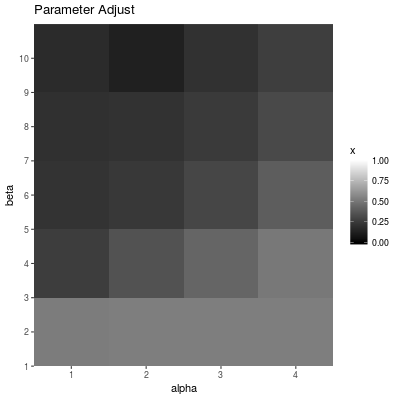
\includegraphics[width=\linewidth]{param_adjust.png} % Figure image
	\caption{Ajuste de parámetros} % Figure caption
	\label{fig:ajuste1} % Label for referencing with \ref{bear}
\end{figure}

\begin{figure}
	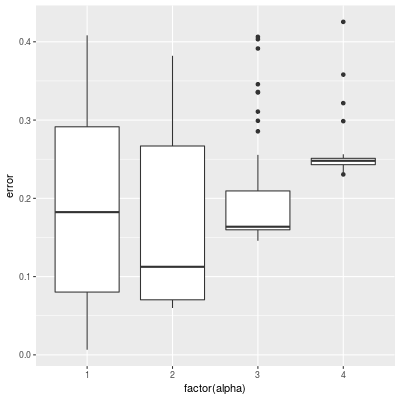
\includegraphics[width=\linewidth]{calibrate_complete_beta10_iter20000_tests50.png} % Figure image
	\caption{Ajuste de parámetros} % Figure caption
	\label{fig:ajuste2} % Label for referencing with \ref{bear}
\end{figure}

\subsection{Grafos completos}

Los grafos completos son aquellos en los que todo par de nodos está 
conectado por un eje. Esta familia es importante en el contexto del 
problema que estamos analizando porque a medida que crece el tamaño de 
la instancia del grafo de input, la \emph{$\alpha$-norma} estima mejor a 
la proyección ortogonal de $f$ sobre el subespacio generado por las 
columnas de las matrices de incidencia dirigida. Más específicamente, 
el ángulo entre dos columnas de una matriz de incidencia dirigida puede 
calcularse mediante la expresión:

$$cos(d_i,d_j) = \frac{d_i d_j}{\|d_i\| \ \|d_j\|} = 
\frac{d_i d_j}{deg(v_i) \ deg(v_j)}$$

\noindent donde $cos(d_i,d_j)$ es el coseno del ángulo entre las columnas de $D$ 
correspondientes a los nodos $v_i$ y $v_j$ del grafo. A medida que el 
grado de los nodos crece, el coseno tiende a $0$, o sea: las columnas 
de $D$ se van volviendo más ortogonales.

\smallskip

En este caso, consideramos tres tipos de instancias de grafos 
completos: de 100, 200 y 400 nodos. Para cada tipo de instancia, se 
hicieron 20 experimentos, cada uno de los cuales se ejecutó durante 
$2 . 10^4$ iteraciones. Es importante notar que la cantidad de ejes de 
un grafo completo es del orden de $n^2$ (donde $|V| = n$).  La figura 
\ref{fig:complete} muestra la media del error en función de la cantidad 
de iteraciones para cada tipo de instancia. Se observa una velocidad de 
convergencia aceptable.


\begin{figure}
	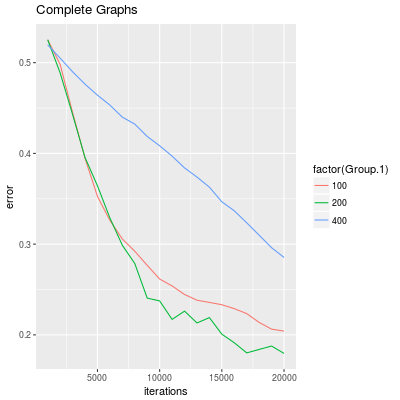
\includegraphics[width=\linewidth]{complete_graphs.png} % Figure image
	\caption{Grafos completos} % Figure caption
	\label{fig:complete} % Label for referencing with \ref{bear}
\end{figure}

\subsection{Ciclos simples}

Los grafos que definen ciclos simples también representan una familia 
de interés. En este caso, como cada nodo tiene solamente dos vecinos, 
la columna de una matriz de incidencia dirigida asociada a un cierto 
nodo, es ortogonal a todas las demás columnas excepto a las asociadas a 
los dos nodos vecinos. En ese caso, el ángulo que forman dos columnas
asociadas a dos nodos vecinos es $\frac{2\pi}{3}$. En esta familia de 
grafos la cantidad de ejes es del orden de $|V| = n$.

\smallskip

En este caso consideramos tres tipos de instancias de ciclos simples: 
de 1000, 2000 y 4000 nodos. Para cada tipo de instancia, se hicieron 
20 experimentos, cada uno de los cuales se ejecutó durante 500 
iteraciones. La figura \ref{fig:cycle} muestra la media del error en 
función de la cantidad de iteraciones para cada tipo de instancia. 
También en este caso, se observa una velocidad de convergencia 
aceptable.

\smallskip

Es importante mencionar que en este caso, la limitación que existe para 
procesar instancias con una mayor cantidad de ejes es la resolución del 
sistema laplaciano $Lx = D^t f$. La matriz $L$ es de tamaño $n \times 
n$, eso impone un límite a esta implementación. Una implementación 
paralelizada de la resolución del sistema lineal permitiría que el 
algoritmo escale sin limitaciones.

\begin{figure}
	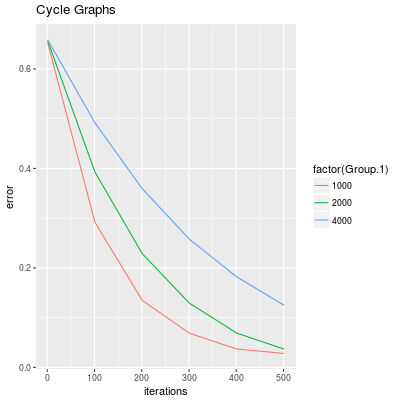
\includegraphics[width=\linewidth]{cycle_graphs.png} % Figure image
	\caption{Ciclos simples} % Figure caption
	\label{fig:cycle} % Label for referencing with \ref{bear}
\end{figure}

\subsection{Mallas poligonales}

\begin{figure}
	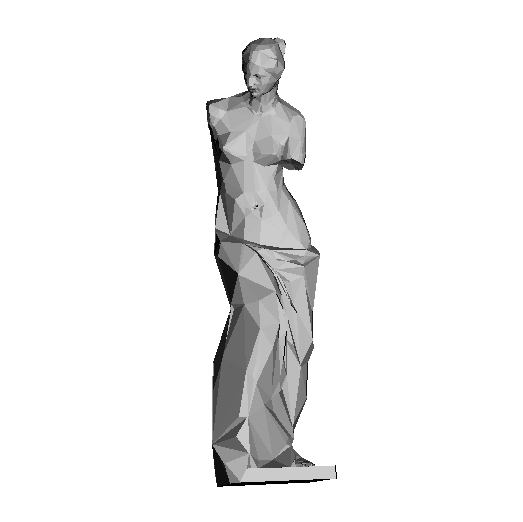
\includegraphics[scale=.21]{venusv_solid.jpg} % Figure image
	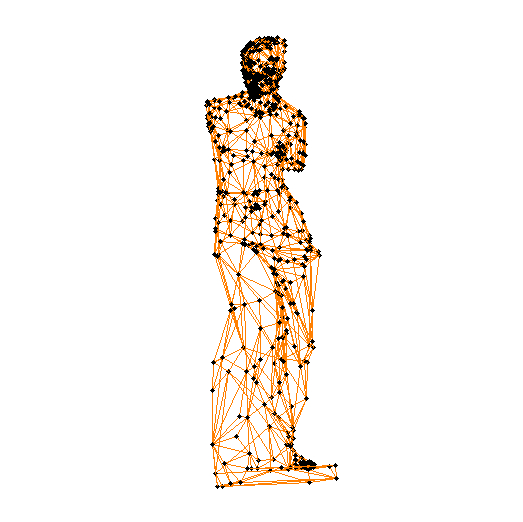
\includegraphics[scale=.21]{venusv_graph.jpg} % Figure image
	\caption{\textbf{venus}: malla poligonal y su grafo subyacente}% Figure caption
	\label{fig:venus} % Label for referencing with \ref{bear}
\end{figure}

\begin{figure}
	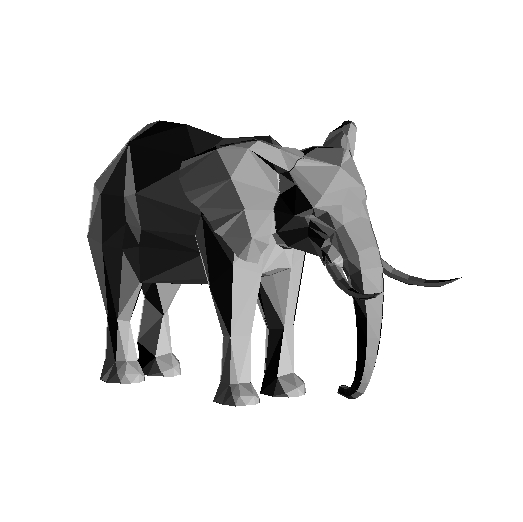
\includegraphics[scale=.21]{elephav_solid.jpg} % Figure image
	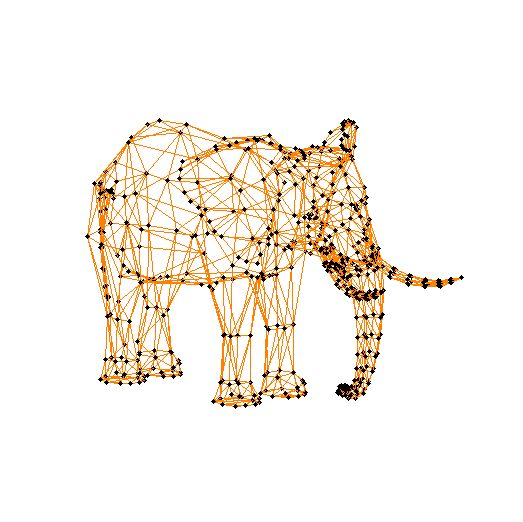
\includegraphics[scale=.21]{elephav_graph.jpg} % Figure image
	\caption{\textbf{elephant}: malla poligonal y su grafo subyacente}% Figure caption
	\label{fig:elephant} % Label for referencing with \ref{bear}
\end{figure}

\begin{figure}
	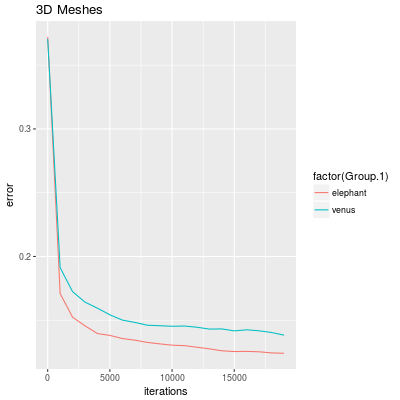
\includegraphics[width=\linewidth]{3dmeshes.png} % Figure image
	\caption{Mallas poligonales}% Figure caption
	\label{fig:meshes} % Label for referencing with \ref{bear}
\end{figure}

\begin{table}
	\caption{Mallas poligonales}
	\centering
	\begin{tabular}{llr}
		\toprule
		malla & $|V|$ & $|E|$ \\
		\midrule
		venus & 819 & 2452 \\
		elephant & 623 & 1759 \\
		\bottomrule
		\label{tab:meshes}
	\end{tabular}
\end{table}

Recordemos que las \textit{mallas poligonales} 
permiten representar superficies inmersas en el espacio tridimensional. 
Las caras son aproximaciones lineales de pequeñas vecindades de la 
superficie. Y el grafo subyacente de una malla describe los bordes de 
las caras. 

\smallskip

En este caso empleamos dos superficies compactas para evaluar el 
algoritmo: \emph{venus} (figura \ref{fig:venus}) y \emph{elephant} 
(figura \ref{fig:elephant}). La tabla \ref{tab:meshes} detalla la 
información de los grafos ($G=(V,E)$) de ambas mallas.

\smallskip

Para cada malla se hicieron 20 experimentos, cada uno de los cuales se 
ejecutó durante $2.10^4$ iteraciones. La figura \ref{fig:meshes} 
muestra la media del error en función de la cantidad de iteraciones. En 
estos casos observamos que inicialmente la convergencia es muy rápida, 
pero a partir de un cierto punto se estabiliza. Este hecho da 
indicios de que esta estrategia debería complementarse con otra que 
permita refinar la mejor solución encontrada.

%venusv.wrl  -> nV: 819 nE: 2452
%elephant.wrl -> nV: 623 nE: 1759

\section{Conclusiones y Trabajo futuro}

En este trabajo abordamos un problema que denominamos \emph{integración 
en grafos} que ``integra'' (en términos analíticos) un dato 
diferencial en los ejes. Este enfoque permite resolver distintos tipos 
de problemas diferenciales que se modelen con grafos. El algoritmo 
metaheurístico que planteamos está basado en comparar \emph{matrices 
de incidencia dirigida} asociadas al grafo de input. Para ello 
consideramos un criterio que denominamos \emph{$\alpha$-norma} vinculado 
a la proyección ortogonal del vector que representa al dato diferencial 
sobre el subespacio generado por las columnas de las matrices de 
incidencia dirigida.

\bigskip

Evaluamos el algoritmo en instancias de tres familias de grafos: grafos 
completos, ciclos simples y mallas poligonales. Y observamos que se comporta 
adecuadamente dado que converge a una solución aproximada del problema 
en un tiempo razonable. No obstante, hay que remarcar que para ciertas 
instancias de input, a partir de cierto punto el algoritmo se 
estabiliza entorno a un error de $0.1$; esto sugiere que la técnica que 
presentamos en este trabajo debería complementarse con otra para 
refinar la solución.

\bigskip

El algoritmo es simple, por lo cual es posible paralelizarlo de modo 
horizontal y procesar instancias de mayor tamaño mediante técnicas 
de procesamiento distribuido (ej.: \emph{map-reduce}).

\bigskip

En la implementación que presentamos, la mayor limitación está 
relacionada a la resolución de \emph{sistemas laplacianos}, es decir: 
sistemas lineales $Lx=b$ en los que $L$ es una \emph{matriz 
laplaciana}. Actualmente hay importantes líneas de trabajo abordando 
nuevas metodologías iterativas que reducen el tiempo de 
procesamiento de este tipo de sistemas. En una a futura implementación
 sería importante incorporar estos enfoques. 

\bigskip

Por último habría que formalizar adecuadamente los argumentos 
estadísticos por los cuales la $\alpha$-norma es una aproximación 
razonable de la proyección ortogonal de un vector sobre un subespacio.

% An example of a floating figure using the graphicx package.
% Note that \label must occur AFTER (or within) \caption.
% For figures, \caption should occur after the \includegraphics.
% Note that IEEEtran v1.7 and later has special internal code that
% is designed to preserve the operation of \label within \caption
% even when the captionsoff option is in effect. However, because
% of issues like this, it may be the safest practice to put all your
% \label just after \caption rather than within \caption{}.
%
% Reminder: the "draftcls" or "draftclsnofoot", not "draft", class
% option should be used if it is desired that the figures are to be
% displayed while in draft mode.
%
%\begin{figure}[!t]
%\centering
%\includegraphics[width=2.5in]{myfigure}
% where an .eps filename suffix will be assumed under latex, 
% and a .pdf suffix will be assumed for pdflatex; or what has been declared
% via \DeclareGraphicsExtensions.
%\caption{Simulation results for the network.}
%\label{fig_sim}
%\end{figure}

% Note that the IEEE typically puts floats only at the top, even when this
% results in a large percentage of a column being occupied by floats.


% An example of a double column floating figure using two subfigures.
% (The subfig.sty package must be loaded for this to work.)
% The subfigure \label commands are set within each subfloat command,
% and the \label for the overall figure must come after \caption.
% \hfil is used as a separator to get equal spacing.
% Watch out that the combined width of all the subfigures on a 
% line do not exceed the text width or a line break will occur.
%
%\begin{figure*}[!t]
%\centering
%\subfloat[Case I]{\includegraphics[width=2.5in]{box}%
%\label{fig_first_case}}
%\hfil
%\subfloat[Case II]{\includegraphics[width=2.5in]{box}%
%\label{fig_second_case}}
%\caption{Simulation results for the network.}
%\label{fig_sim}
%\end{figure*}
%
% Note that often IEEE papers with subfigures do not employ subfigure
% captions (using the optional argument to \subfloat[]), but instead will
% reference/describe all of them (a), (b), etc., within the main caption.
% Be aware that for subfig.sty to generate the (a), (b), etc., subfigure
% labels, the optional argument to \subfloat must be present. If a
% subcaption is not desired, just leave its contents blank,
% e.g., \subfloat[].


% An example of a floating table. Note that, for IEEE style tables, the
% \caption command should come BEFORE the table and, given that table
% captions serve much like titles, are usually capitalized except for words
% such as a, an, and, as, at, but, by, for, in, nor, of, on, or, the, to
% and up, which are usually not capitalized unless they are the first or
% last word of the caption. Table text will default to \footnotesize as
% the IEEE normally uses this smaller font for tables.
% The \label must come after \caption as always.
%
%\begin{table}[!t]
%% increase table row spacing, adjust to taste
%\renewcommand{\arraystretch}{1.3}
% if using array.sty, it might be a good idea to tweak the value of
% \extrarowheight as needed to properly center the text within the cells
%\caption{An Example of a Table}
%\label{table_example}
%\centering
%% Some packages, such as MDW tools, offer better commands for making tables
%% than the plain LaTeX2e tabular which is used here.
%\begin{tabular}{|c||c|}
%\hline
%One & Two\\
%\hline
%Three & Four\\
%\hline
%\end{tabular}
%\end{table}


% Note that the IEEE does not put floats in the very first column
% - or typically anywhere on the first page for that matter. Also,
% in-text middle ("here") positioning is typically not used, but it
% is allowed and encouraged for Computer Society conferences (but
% not Computer Society journals). Most IEEE journals/conferences use
% top floats exclusively. 
% Note that, LaTeX2e, unlike IEEE journals/conferences, places
% footnotes above bottom floats. This can be corrected via the
% \fnbelowfloat command of the stfloats package.


% conference papers do not normally have an appendix

% use section* for acknowledgment
\ifCLASSOPTIONcompsoc
  % The Computer Society usually uses the plural form
  \section*{Agradecimientos}
\else
  % regular IEEE prefers the singular form
  \section*{Agradecimiento}
\fi

Queremos agradecer al proyecto UndavCyT 2014 ``Especificaciones formales 
tempranas del comportamiento de sistemas de software''.

\bigskip

Los autores queremos agradecer al Prof. Gabriel Taubin por plantearnos 
el problema de integración de formas diferenciales en el contexto de 
mallas poligonales y por su generosa disposición a responder nuestras 
preguntas. Asimismo queremos agradecer al Prof. Fernando Cukierman por 
guiar nuestro estudio en el área de geometría diferencial.


% trigger a \newpage just before the given reference
% number - used to balance the columns on the last page
% adjust value as needed - may need to be readjusted if
% the document is modified later
%\IEEEtriggeratref{8}
% The "triggered" command can be changed if desired:
%\IEEEtriggercmd{\enlargethispage{-5in}}

% references section

% can use a bibliography generated by BibTeX as a .bbl file
% BibTeX documentation can be easily obtained at:
% http://mirror.ctan.org/biblio/bibtex/contrib/doc/
% The IEEEtran BibTeX style support page is at:
% http://www.michaelshell.org/tex/ieeetran/bibtex/
%\bibliographystyle{IEEEtran}
% argument is your BibTeX string definitions and bibliography database(s)
%\bibliography{IEEEabrv,../bib/paper}
%
% <OR> manually copy in the resultant .bbl file
% set second argument of \begin to the number of references
% (used to reserve space for the reference number labels box)

\renewcommand\refname{Referencias}

\begin{thebibliography}{1}

\bibitem[Taubin et al., 2002]{BMMRT:2002}
Bernardini F., Martin I., Mittleman J., Rushmeier H., Taubin G.,
\newblock \textit{Building a Digital Model of Michelangelo's Florentine Pieta'}
\newblock IEEE Computer Graphics and Applications.

\bibitem[Botsch, Kobbelt, Pauly, Alliez, Lévy, 2010]{BKPAL:2010}
Botsch M., Kobbelt L., Pauly M., Alliez P., Lévy B.,
\newblock \textit{Polygon Mesh Processing}
\newblock A. K. Peters, 2010.

\bibitem[Crispell, Mundy, Taubin, 2008]{CMT:2008}
Crispell D., Mundy J., Taubin G.,
\newblock \textit{Parallax-Free Aerial Video Registration}
\newblock British Machine Vision Conference 2008.

\bibitem[Desbrun, Kanso, Tong, 2006]{DKT:2006}
Desbrun M., Kanso E., Tong Y.,
\newblock \textit{Discrete differential forms for computational 
modeling}
\newblock Proceeding SIGGRAPH '06 ACM SIGGRAPH 2006 Courses Pages 
39-54 .
 
\bibitem[Gendrau, Potvin, 2010]{GP:2010}
Gendreau M. and Potvin J., 
\newblock \textit{Handbook of Metaheuristics}, 
\newblock Springer, 2010.

\bibitem[Harari, 1969]{Harari:1969}
Harary F., 
\newblock \textit{Graph Theory}, 
\newblock Addison-Wesley, 1969.

\bibitem[Hatcher, 2004]{Hatcher:2004}
Hatcher A., 
\newblock \textit{Algebraic Topology}, 
\newblock Cambridge University Press.

\bibitem[Koutis, Miller, Peng, 2010]{KMP:2010}
Koutis I., Miller G. L. and Peng R., 
\newblock \textit{Approaching optimality for solving sdd linear systems}, 
\newblock 51st Annual Symposium on Foundations of Computer Science, IEEE, 
2010, pp. 235-244.

\bibitem[Lanman, Raskar, Agrawal, Taubin, 2008]{LRAT:2008}
Lanman D., Raskar R., Agrawal A., Taubin G., 
\newblock \textit{Shield Fields: Modeling and Capturing 3D Occluders}, 
\newblock ACM Transactions on Graphics (TOG), Vol 27, Issue 5, December 
2008, Siggraph Asia Proceedings.

\bibitem[REVEAL]{REVEAL}
\newblock Reconstruction and ExploratoryVisualization: Engineering 
meets Art / ArchaeoLogy.

\bibitem[Ronfard, Taubin, 2007]{RT:2007}
Ronfard R., Taubin G., 
\newblock \textit{Introducing 3D Cinematography}, 
\newblock IEEE Computer Graphics and Applications (pp. 18-20).

\bibitem[Saad, 2007]{Saad:2007}
Saad Y., 
\newblock \textit{Iterative methods for sparse linear systems}, 
\newblock SIAM, 2007.

\bibitem[Spielman, 2010]{Spielman:2010}
Spielman D. A.,
\newblock \textit{Algorithms, graph theory, and linear equations in laplacian 
matrices}, 
\newblock Proceedings of the International Congress of Mathematicians, vol. 4, 
2010, pp. 2698-2722.

\bibitem[Spielman, Teng, 2004]{ST:2004}
Spielman D. A. and Shang-Hua Teng,
\newblock \textit{Nearly-linear time algorithms for graph partitioning, graph 
sparsification, and solving linear systems}, 
\newblock Proceedings of the thirty-sixth annual ACM symposium on Theory of 
Computing, ACM, 2004, pp. 81-90.

\bibitem[Spivak, 1965]{S:1965}
Spivak M.,
\newblock \textit{Calculus on Manifolds},
\newblock W. A. Benjamin.

\bibitem[Talbi, 2009]{Talbi:2009}
Talbi E.G., 
\newblock \textit{Metaheuristics: from design to implementation}, 
\newblock Wiley, 2009.

\bibitem[Taubin, Cooper, 1992]{TC:1992}
Taubin G., Cooper D.B., 
\newblock \textit{2D and 3D Object Recognition and Positioning with 
Algebraic Invariants and Covariants}, 
\newblock Academic Press.

\bibitem[Teng, 2010]{Teng:2010}
Shang-Hua Teng,
\newblock \textit{The laplacian paradigm: Emerging algorithms for massive 
graphs}, 
\newblock Theory and Applications of Models of Computation, Lecture Notes in 
Computer Science, vol. 6108, 2010, pp. 2-14.

\bibitem[Tu, 2008]{T:2008}
Tu, L. W. 
\newblock \textit{An Introduction to Manifolds},
\newblock Springer.

\bibitem[Ward, Kincaid, 2009]{WK:2009}
Ward C., Kincaid D., 
\newblock \textit{Linear Algebra: Theory and Applications}
\newblock Sudbury, Ma: Jones and Bartlett. pp. 544, 558.

\bibitem[Zhao, Taubin, 2009]{ZT:2009}
Zhao Y., Taubin G., 
\newblock \textit{Real-Time High Definition Stereo on GPGPU using 
Progressive Multi-Resolution Adaptive Windows}
\newblock NVIDIA Research Summit 2009, NVIDIA GPU Technology Conference.

\end{thebibliography}

% that's all folks

\end{document}


%[17] Taubin G., Cooper D.B. (1992) 2D and 3D Object Recognition and Positioning with Algebraic Invariants and Covariants. Academic Press.

%[18] Lanman D., Crispell D.,Taubin G. (2009) Surround Structured Lighting: 3-D Scanning with Orthographic Illumination. Computer Vision and Image Understanding (CVIU), Volume 113, Issue 11,(pp 1107-1117).

%[19] Leotta M., Vandergon A., Taubin G. (2008) 3D Slit Scanning with Planar Constraints. Computer Graphics Forum, Volume 27, Number 8, (pp. 2066-2080).

%[20] Lanman D., Raskar R., Agrawal A., Taubin G. (2008) Shield Fields: Modeling and Capturing 3D Occluders. ACM Transactions on Graphics (TOG), Vol 27, Issue 5, December 2008, Siggraph Asia Proceedings.

%[21] Osman Ulusoy A., Calakli F., Taubin G. (2009) One Shot Scanning Using DeBrujin Spaced Grids. IEEE International Workshop on 3-D Digital Imaging and Modeling (3DIM'09), Kyoto, Japan

%[22] Ronfard R., Taubin G. (2007) Introducing 3D Cinematography. IEEE Computer Graphics and Applications (pp. 18-20).

%[23] Bernardini F., Martin I., Mittleman J., Rushmeier H., Taubin G. (2002) Building a Digital Model of Michelangelo's Florentine Pieta'. IEEE Computer Graphics & Applications.

%[24] Zhao Y., Taubin G. (2009) Real-Time High Definition Stereo on GPGPU using Progressive Multi-Resolution Adaptive Windows. NVIDIA Research Summit 2009, NVIDIA GPU Technology Conference.

%[25] Bergou A. J., Swartz S., Breuer K., Taubin G. 3D Reconstruction of Bat Flight Kinematics from Sparse Multiple Views

%[26] Crispell D., Mundy J., Taubin G. (2008) Parallax-Free Aerial Video Registration. British Machine Vision Conference 2008.

%[27] Andaló F.A., Calakli F., Taubin G., Goldenstein S. Accurate 3D Footwear Impression Recovery From Photographs
% 






